\documentclass[../main.tex]{subfiles}

\begin{document}

RDF es un lenguaje de modelado para describir recursos en la web. RDF permite modelar recursos (datos) y sus relaciones mediante un grafo dirigido.

\hfill

\subsection{Clases RDF}

Se ha tenido que desarrollar un mapa de clases que están relacionados mediante propiedades de datos. Definiendo las clases, operaciones:

\hfill

\begin{figure}[ht]
    \centering
    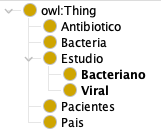
\includegraphics[scale=0.65]{images/clasesport.png}
    \caption{Clases}
    \label{clasesport}
\end{figure}


\begin{figure}[h]
    \centering
    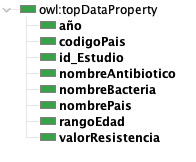
\includegraphics[scale=0.65]{images/porpieddes .png}
    \caption{Relaciones}
    \label{Relaciones}
\end{figure}

El mapa se ha jerarquizado en torno al estudio que se esta realizando, de el parten las relaciones.

\newpage

\subsection{Propiedades RDF}

Para expresar atributos de las clases se han creado propiedades:

\hfill

\begin{figure}[ht]
    \centering
    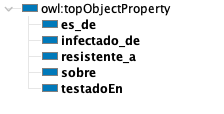
\includegraphics[scale=0.65]{images/operaciones.png}
    \caption{Clases}
    \label{operaciones}
\end{figure}

Estas propiedades complementan a ciertas clases, aportando información sobre ellas. La mayoría se trata de propiedades de una clase a un tipo de dato int o string peor rango de edad se ha declarado como un enumerado.

\hfill

\begin{figure}[ht]
    \centering
    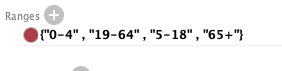
\includegraphics[scale=0.65]{images/reeee.png}
    \caption{Propiedad enumerado}
    \label{reeee}
\end{figure}

La figura final, resultado del confeccionar un modelo con relaciones entre las clases (object properties), es el grafo RDF. 
\begin{figure}[ht]
    \centering
    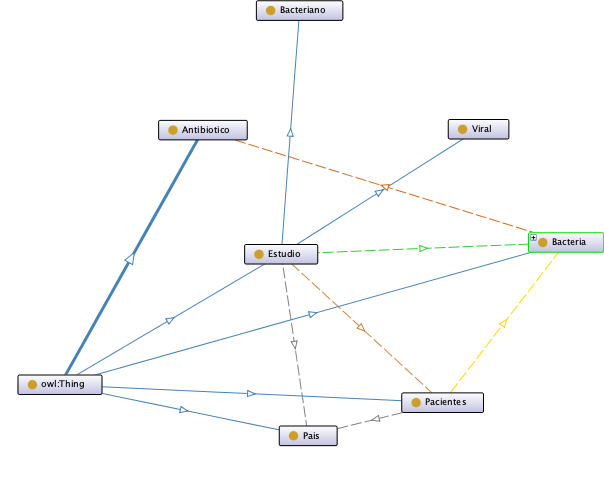
\includegraphics[scale=0.35]{images/rdf graph.png}
    \caption{Grafo RDF}
    \label{rdf graph}
\end{figure}

\subsection{Queries SPARQL}

Para poder acceder al modelo .OWL, se ha creado un prefijo llamado sch que almacena el uri del proyecto. A través de el podremos consultar las propiedades de objetos, de clases y las propias clases.

\subsubsection{Query 1}

Muestra de el id de estudio, el nombre del país donde fue realizado, el nombre de la bacteria con el antibiótico que se testo y el porcentaje de éxito de los estudios por país dado:

\begin{figure}[ht]
    \centering
    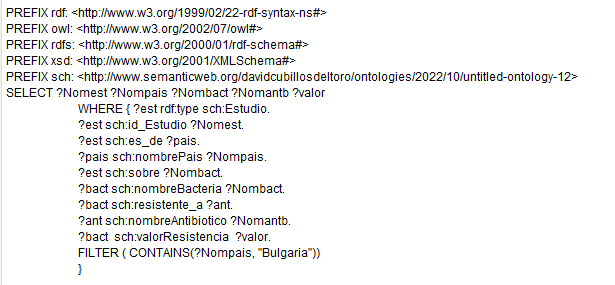
\includegraphics[scale=0.5]{images/sparql-1.PNG}
    \caption{Muestra de los estudios de Bulgaria}
    \label{spark1}
\end{figure}

 

\subsubsection{Query 2}

La segunda query, muy similar a la primera, muestro los datos de todos los estudios ordenándolos ascendentemente por el valor de la resistencia que la bacteria tiene al antibiótico. Muestra los campos: nombre de la bacteria, nombre del antibiótico y el valor propio de la resistencia. 


\begin{figure}[ht]
    \centering
    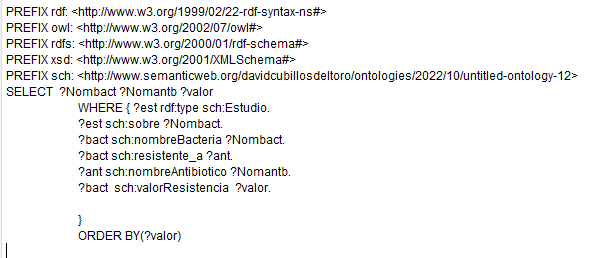
\includegraphics[scale=0.5]{images/sparql-2.PNG}
    \caption{Resistencia de una bacteria a su antibiótico}
    \label{spark2}
\end{figure}
\end{document}